\documentclass[convert = false, tikz]{standalone}
\usepackage[utf8]{inputenc}
\usepackage{tikz}
\usetikzlibrary{automata, positioning, arrows}
 
\usepackage{../../../../style_automata}

% arara: pdflatex
% arara: latexmk: { clean: partial }
\begin{document}
    \tikzset{
    node distance=1.8cm, % specifies the minimum distance between two nodes.
    }
    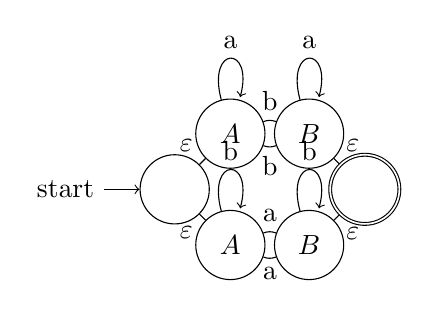
\begin{tikzpicture}
        \node[state, initial] (0) {};
        \node[state, above right of=0] (a) {$A$};
        \node[state, below right of=0] (a2) {$A$};
        \node[state, right of=a] (b2) {$B$};
        \node[state, right of=a2] (b) {$B$};
        \node[state, accepting, below right of=b2] (1) {};
        \draw (0) edge[above left] node{$\varepsilon$} (a)
        (0) edge[below left] node{$\varepsilon$} (a2)
        (a) edge[loop above] node{a} (a)
        (a) edge[above, bend left=20] node{b} (b2)
        (a2) edge[loop above] node{b} (a2)
        (a2) edge[above, bend left=20] node{a} (b)
        (b) edge[loop above] node{b} (b)
        (b) edge[below, bend left=20] node{a} (a2)
        (b2) edge[loop above] node{a} (b2)
        (b2) edge[below, bend left=20] node{b} (a)
        (b2) edge[above right] node{$\varepsilon$} (1)
        (b) edge[below right] node{$\varepsilon$} (1)
        ;
    \end{tikzpicture}
\end{document}
